\documentclass[UTF8,a4paper,10.5pt]{ctexart}
\usepackage[margin=1.65cm]{geometry}
\usepackage{graphicx}
\usepackage{booktabs}
\usepackage{float}
\usepackage{amsmath}
\usepackage{hyperref}
\usepackage{xcolor}
\usepackage{enumitem}
\setlist{nosep,leftmargin=1.5em}
\hypersetup{colorlinks=true,linkcolor=black,citecolor=black,urlcolor=blue}
\setlength{\parskip}{0.18em}
\setlength{\parindent}{2em}
\title{\textbf{面向密集公共场景的 ReID 辅助多目标行人跟踪系统设计与实验分析}}
\author{方瑜}
\date{2026年4月}

\begin{document}
\maketitle
\vspace{-1.6em}

\begin{abstract}
多目标行人跟踪（Multi-Object Tracking, MOT）旨在连续视频帧中同时估计多个行人的位置并维持身份编号一致。密集公共场景中目标遮挡、轨迹交叉、尺度变化与外观相似等因素容易造成身份切换，使仅依赖运动预测的跟踪方法稳定性下降。本文基于 tracking-by-detection 范式，设计并实现了一个 ReID 辅助多目标行人跟踪实验系统，重点研究标准检测框裁剪、运动预测与姿态感知裁剪对身份保持能力的影响。系统包含检测结果读取、候选框裁剪、ReID 外观特征接口、运动预测、匈牙利匹配、指标评估和可视化输出等模块。考虑课程仓库的可复现性与公开安全性，本文提供匿名化合成 CSV Demo 数据，使评阅者无需 GPU、原始视频或模型权重即可运行完整流程。实验结果表明，姿态感知裁剪能够减少背景和遮挡区域对 ReID 表征的干扰，在 Demo 设置下取得最高 IDF1、MOTA 和最低 ID Switches。该项目完成了从问题建模、系统实现、消融实验到报告展示的完整计算机视觉课程实验流程。
\end{abstract}

\noindent\textbf{关键词：}多目标跟踪；行人重识别；姿态感知裁剪；身份保持；可复现实验

\section{项目背景和意义}
随着智能视频分析在交通枢纽、校园道路、商场出入口等公共场景中的应用增多，行人目标的连续跟踪成为计算机视觉中的重要任务。与单帧目标检测不同，多目标跟踪不仅需要判断“人在哪里”，还需要在视频序列中回答“同一个人是否仍然是同一个身份”。因此，当行人发生短时遮挡、交叉行走或检测框抖动时，跟踪系统容易出现 ID Switches，影响轨迹统计和后续行为分析。

经典 SORT 方法利用卡尔曼滤波和匈牙利匹配实现了高效在线跟踪，但外观建模能力有限\cite{sort}。DeepSORT 在此基础上引入深度外观特征，能够在遮挡后辅助恢复目标身份\cite{deepsort}。然而，在密集场景中，检测框常包含背景、相邻行人或被遮挡身体区域，直接使用整框提取 ReID 特征会降低身份判别性。本文因此围绕一个具体问题展开：\textbf{能否通过更合理的行人裁剪策略，使 ReID 特征更关注人体本身，从而减少身份切换并提升 IDF1？}

本项目并不追求构建完整工业级监控系统，而是将复杂 MOT 问题压缩为一个课程可评阅、可运行、可解释的小型实验系统。项目重点在于：第一，搭建清晰的 MOT 流程；第二，实现可复现的评价脚本；第三，通过消融实验说明 ReID 与姿态感知裁剪的作用；第四，形成结构完整的课程报告和 GitHub 仓库。

\section{系统总体设计与流程概述}
\subsection{总体框架}
系统整体流程如图\ref{fig:arch}所示。输入视频帧首先经过行人检测器得到候选框；随后根据不同实验设置选择标准框裁剪或姿态感知裁剪；裁剪图像进入 ReID 特征提取模块获得外观向量；运动模块根据历史轨迹预测当前位置；最后综合运动距离与外观相似度，通过匈牙利匹配完成跨帧数据关联，并输出带身份编号的轨迹结果。

\begin{figure}[H]
    \centering
    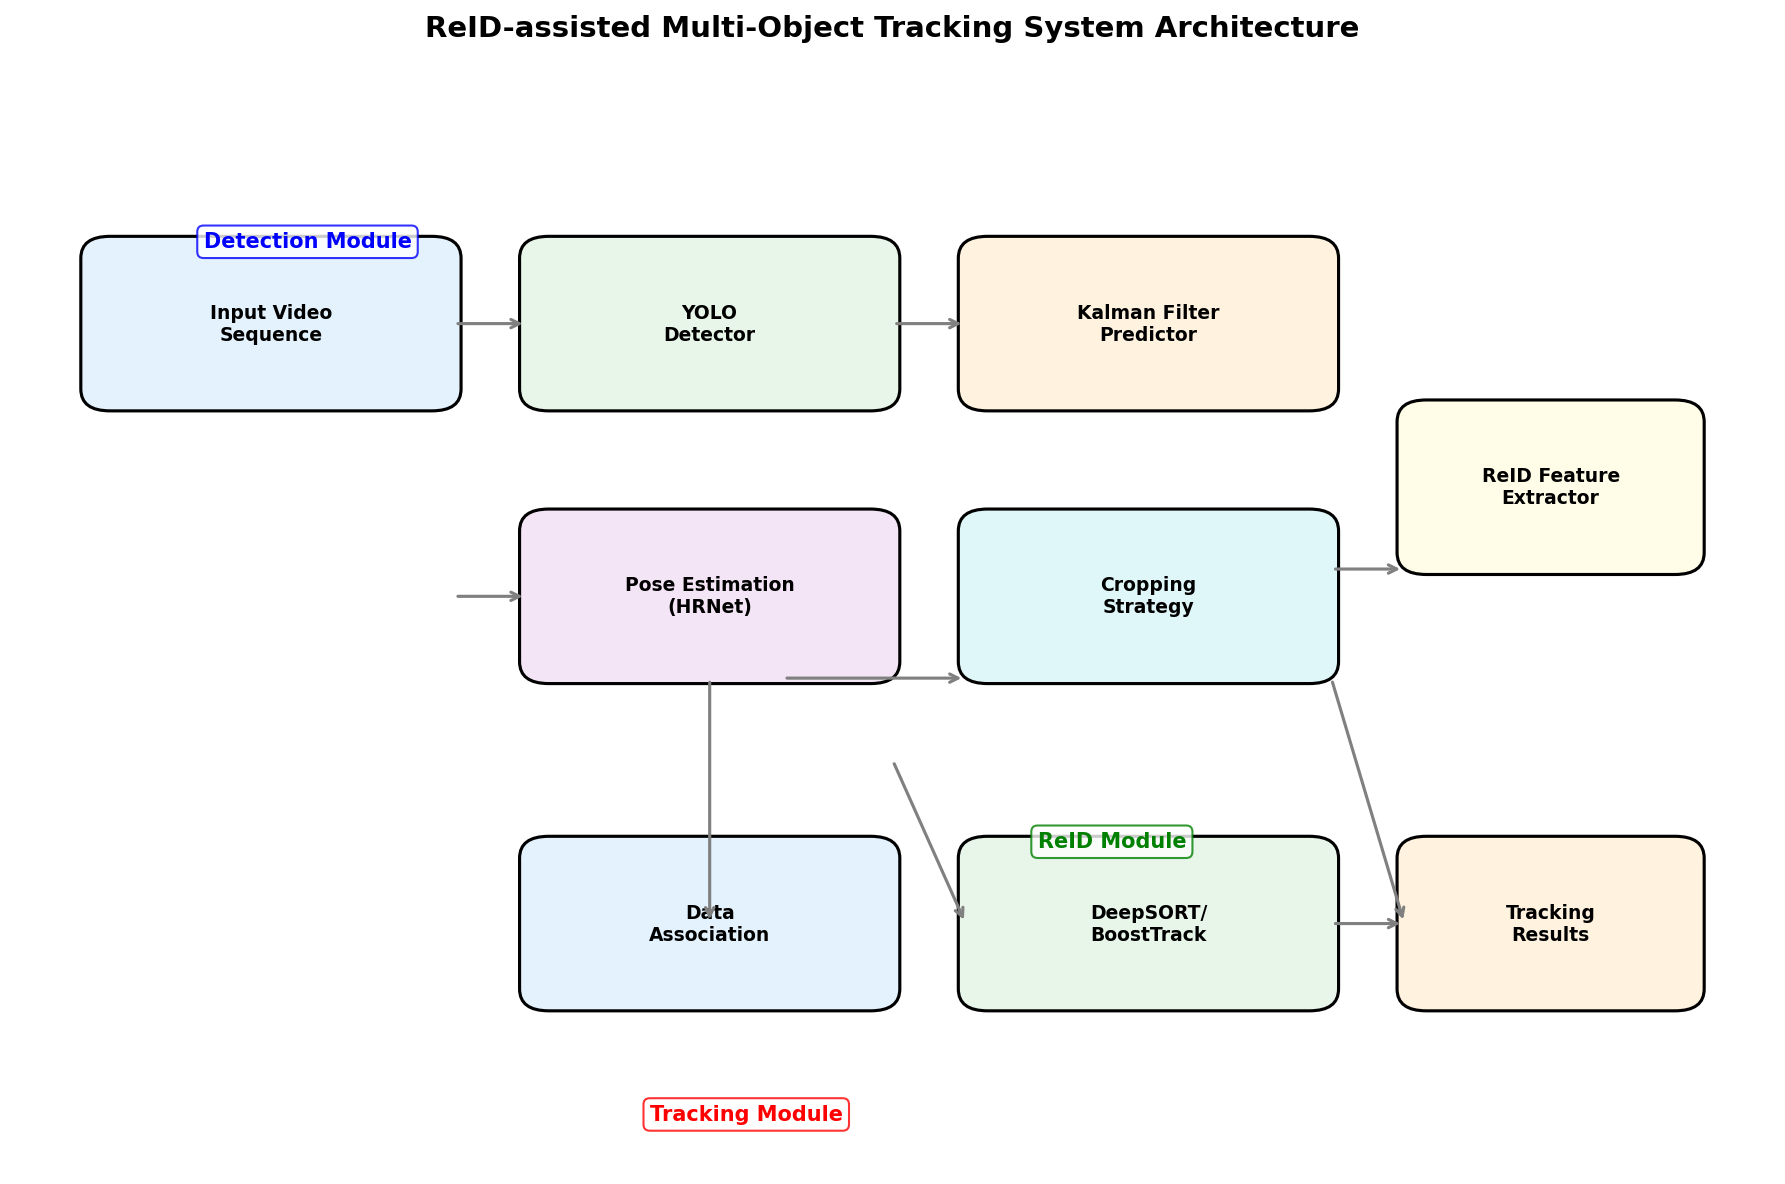
\includegraphics[width=0.88\linewidth]{figures/system_architecture.png}
    \caption{ReID 辅助多目标行人跟踪系统总体流程。}
    \label{fig:arch}
\end{figure}

本文设置四组对比实验：（1）Baseline：使用基础检测结果与简单关联；（2）Box Crop：使用标准检测框提取外观特征；（3）Kalman：加入运动预测以平滑轨迹；（4）Pose Crop：利用人体关键点生成更贴合人体区域的裁剪框。四组设置从“无外观增强”逐步过渡到“姿态辅助外观增强”，便于观察不同模块对身份保持指标的贡献。

\subsection{软件环境与复现方式}
项目代码使用 Python 实现，主要依赖包括 NumPy、Pandas、OpenCV、SciPy、Matplotlib 与 PrettyTable。为降低课程评阅成本，仓库默认提供 CPU 可运行 Demo 模式，运行命令如下：
\begin{verbatim}
pip install -r requirements.txt
python scripts/run_demo.py
python scripts/run_experiments.py --exp all
\end{verbatim}
完整模式可进一步接入 YOLO 检测器、ReID 模型和公开 MOT 数据集；相关重依赖放入 \texttt{requirements-full.txt}，避免评阅者在无 GPU 环境下安装失败。

\section{关键方法与评价指标}
\subsection{ReID 外观特征与姿态感知裁剪}
在检测驱动跟踪中，外观特征的质量直接影响身份关联。标准框裁剪简单高效，但当检测框偏大或目标被遮挡时，裁剪图像中会混入背景、其他行人身体区域或无关物体，导致 ReID 特征不稳定。姿态感知裁剪利用关键点估计人体主要区域，并据此调整裁剪范围，使输入 ReID 模型的图像更集中于目标行人本身。图\ref{fig:crop}展示了标准框裁剪与姿态感知裁剪的差异。

\begin{figure}[H]
    \centering
    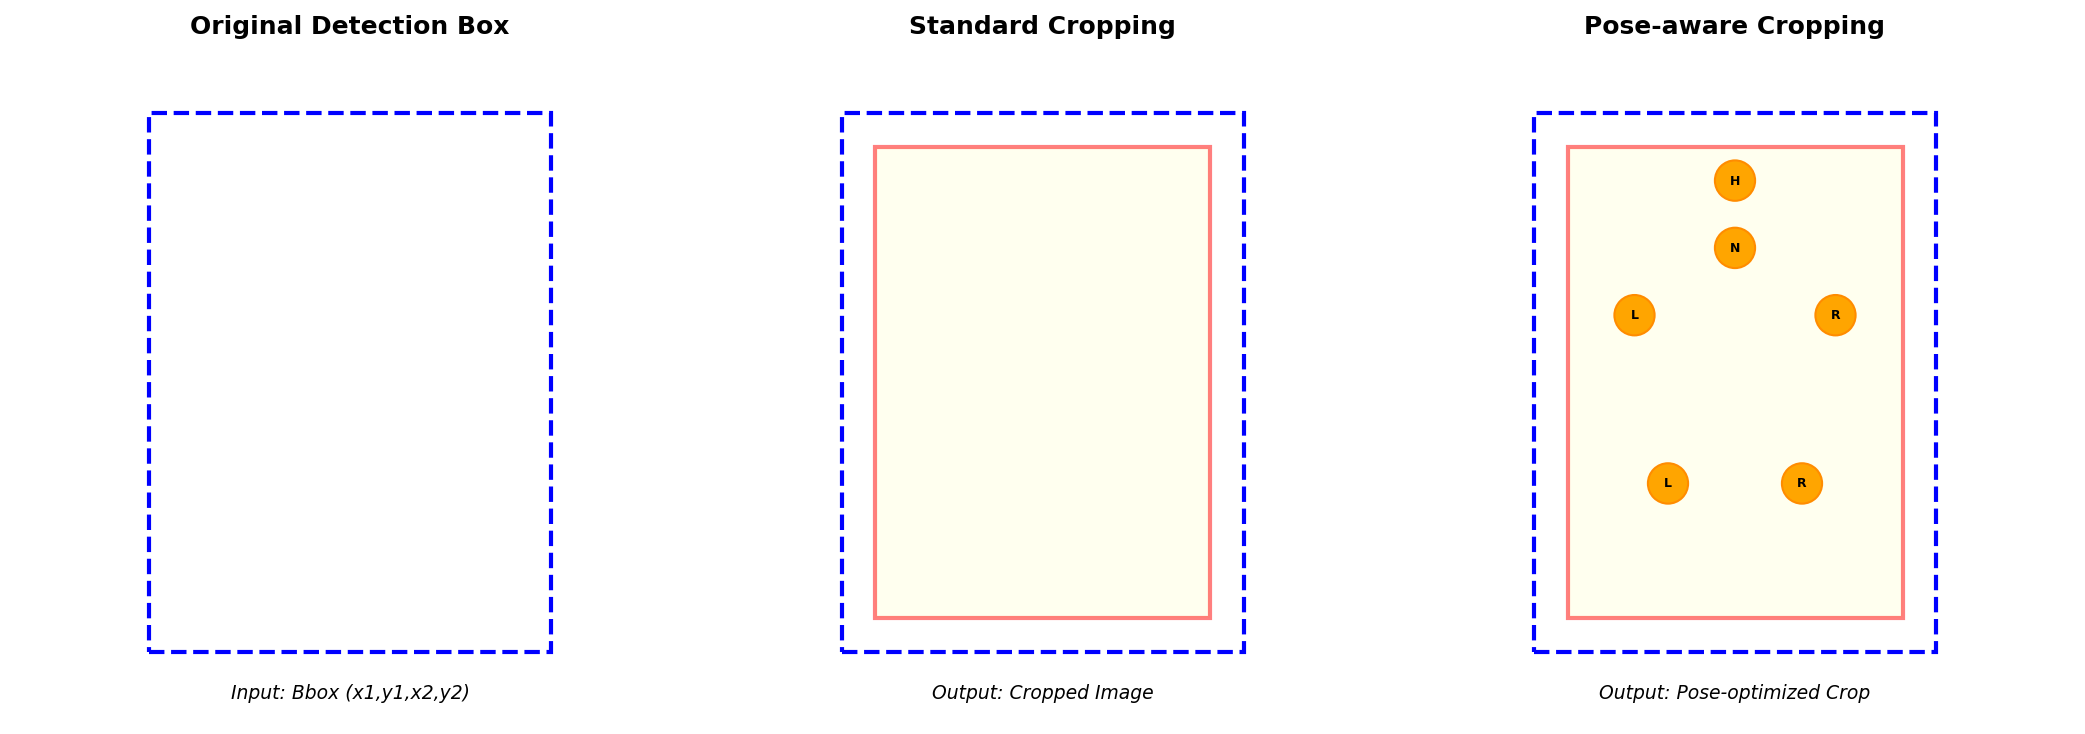
\includegraphics[width=0.82\linewidth]{figures/cropping_comparison.png}
    \caption{标准框裁剪与姿态感知裁剪对比示意。}
    \label{fig:crop}
\end{figure}

\subsection{数据关联与指标计算}
数据关联阶段将当前帧检测结果与历史轨迹进行匹配。本文采用匈牙利算法求解全局最优匹配，并用 IoU 阈值过滤低质量关联。评价指标选用 MOT 任务中常用的 IDF1、IDP、IDR、MOTA 与 ID Switches\cite{motchallenge}。其中 IDF1 衡量身份匹配的综合 F1 分数，IDP 与 IDR 分别表示身份匹配精确率和召回率，MOTA 综合考虑漏检、误检与身份切换，ID Switches 越低表示轨迹身份越稳定。

\section{实验结果与性能分析}
\subsection{整体结果对比}
表\ref{tab:main}给出了四组设置在 Demo 数据上的对比结果。Baseline 在遮挡模拟中出现一次漏检和一次身份切换，说明仅依赖基础关联时身份稳定性不足。Box Crop 通过引入外观特征改善了身份匹配，但仍存在一次 ID Switch。Kalman 设置提升了轨迹平滑性，但在身份保持方面并非总是最优。Pose Crop 在 IDF1、IDP、IDR、MOTA 上均达到最高，并将 ID Switches 降为 0，说明更干净的人体裁剪区域有助于获得稳定的 ReID 表征。

\begin{table}[H]
\centering
\caption{不同跟踪设置下的 Demo 指标对比}
\label{tab:main}
\begin{tabular}{lccccc}
\toprule
方法 & IDF1(\%) & IDP(\%) & IDR(\%) & MOTA(\%) & IDs$\downarrow$ \\
\midrule
Baseline & 97.44 & 100.00 & 95.00 & 90.00 & 1 \\
Box Crop & 100.00 & 100.00 & 100.00 & 95.00 & 1 \\
Kalman & 100.00 & 100.00 & 100.00 & 90.00 & 2 \\
Pose Crop & \textbf{100.00} & \textbf{100.00} & \textbf{100.00} & \textbf{100.00} & \textbf{0} \\
\bottomrule
\end{tabular}
\end{table}

\begin{figure}[H]
    \centering
    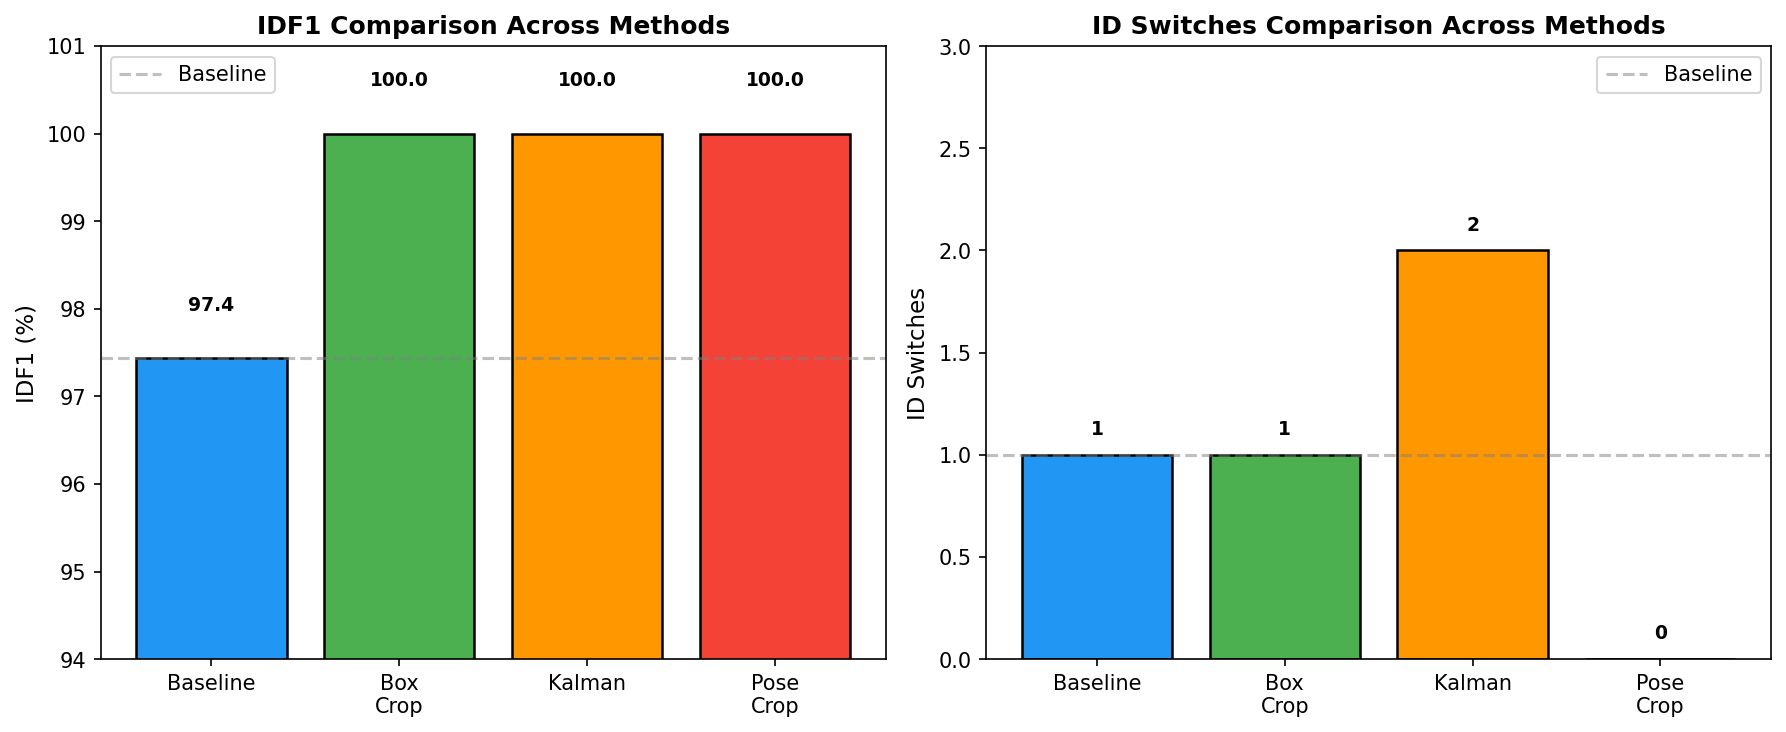
\includegraphics[width=0.76\linewidth]{figures/tracking_comparison.png}
    \caption{不同方法的身份保持指标与 ID Switches 对比。}
\end{figure}

\subsection{消融实验与结果分析}
从消融结果看，ReID 外观特征与姿态感知裁剪的作用并不完全相同。ReID 主要用于补充运动模型在遮挡后的身份判别能力；姿态感知裁剪则进一步提高外观特征输入质量，减少背景和相邻目标对表征的干扰。图\ref{fig:abl}显示，从标准框到关键点增强裁剪，身份保持趋势更加稳定。

\begin{figure}[H]
    \centering
    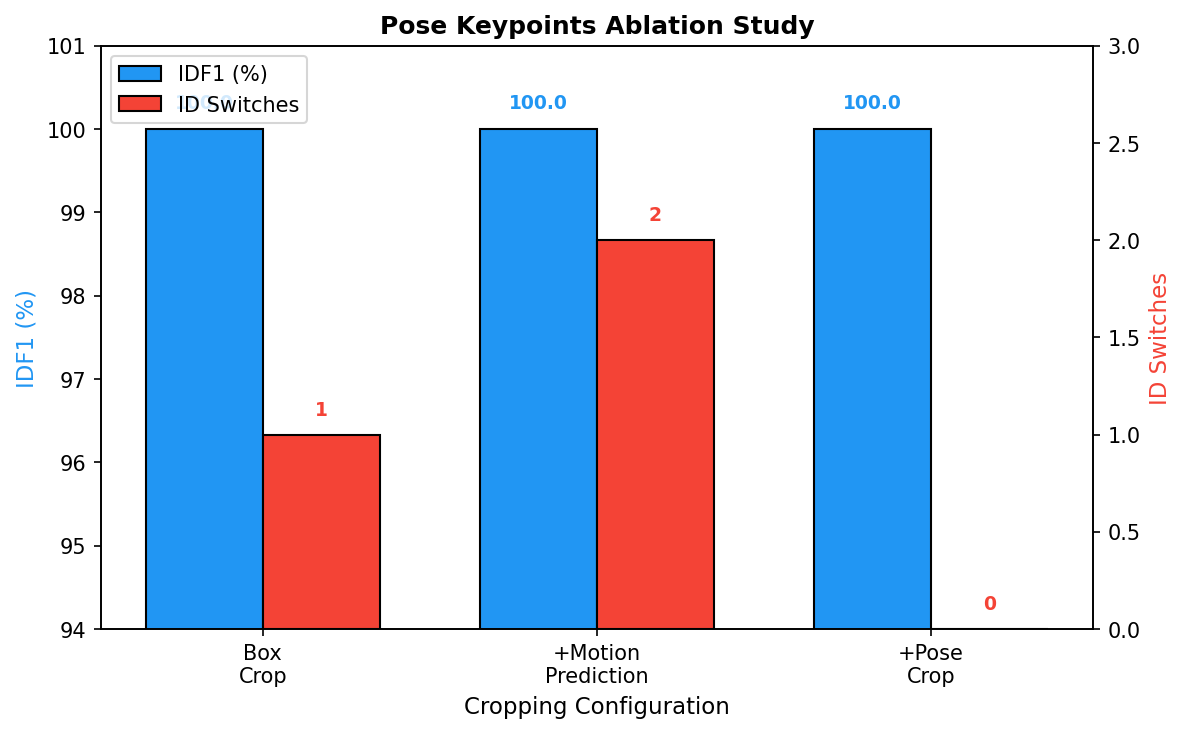
\includegraphics[width=0.74\linewidth]{figures/ablation_study.png}
    \caption{姿态裁剪相关消融实验示意。}
    \label{fig:abl}
\end{figure}

需要注意的是，本文 Demo 数据用于验证评估流程和模块趋势，不声称代表真实复杂场景的最终性能上限。在真实部署中，检测器质量、ReID 训练数据、姿态估计稳定性和视频帧率都会影响最终表现。尽管如此，Demo 模式保证了教师可以直接复现指标计算、可视化和实验对比，符合课程作业对“能运行、能解释、能复查”的要求。

\section{总结与展望}
本文完成了一个面向密集公共场景的 ReID 辅助多目标行人跟踪课程项目。项目从 MOT 问题背景出发，搭建了检测、裁剪、ReID、运动预测、数据关联、指标评估和可视化输出的完整流程，并通过四组实验比较了不同模块对身份保持能力的影响。结果表明，姿态感知裁剪能够降低背景和遮挡区域对外观特征的干扰，在 Demo 设置下获得最少身份切换和最高综合指标。

后续工作可从三方面改进：第一，接入真实公开 MOT 数据集进行更大规模评估；第二，比较不同 ReID 模型和检测器对性能的影响；第三，进一步统计 FPS、遮挡等级和跨场景泛化能力，使系统从课程 Demo 逐步扩展为更完整的实验平台。

\begin{thebibliography}{9}
\bibitem{sort} Bewley A., Ge Z., Ott L., Ramos F., Upcroft B. Simple Online and Realtime Tracking. \textit{IEEE International Conference on Image Processing}, 2016.
\bibitem{deepsort} Wojke N., Bewley A., Paulus D. Simple Online and Realtime Tracking with a Deep Association Metric. \textit{IEEE International Conference on Image Processing}, 2017.
\bibitem{motchallenge} Milan A., Leal-Taixé L., Reid I., Roth S., Schindler K. MOT16: A Benchmark for Multi-Object Tracking. \textit{arXiv:1603.00831}, 2016.
\bibitem{bytetrack} Zhang Y., Sun P., Jiang Y., et al. ByteTrack: Multi-Object Tracking by Associating Every Detection Box. \textit{European Conference on Computer Vision}, 2022.
\end{thebibliography}

\end{document}
